\subsection{Dalvik EXecutionable File} \label{subsection:android-dalvik}
%START TEXT INPUT
This is my real text! Rest might be copied or not be checked!
%START TEXT INPUT

%
AUFBAU DEX
DVM is register based. Registers are considered 32 bits wide to store values such as integers or floating point numbers. Adjacent register pairs are used to store 64-bit values\newline
dest-then-source ordering for its arguments\newline
there are 218 used valid opcodes in Dalvik bytecode -see- QUELLE \newline

Due to its simplicity over bytecode for other architectures as well as the little protection applied in practice, Dalvik bytecode is currently an easy target for the reverse engineer.

VERGLEICHSBILD JAVA---DEX\cite{ehringerDalvik}\newline
Each .class file has its own heterogeneous constant pool which may contain duplicating data, BEISPIEL, memory efficiency of a .dex file comes primarily from the type-specific constant pools used to store the data, BEISPIEL,\newline
significantly more references within a .dex file compared to a .class file\cite{ehringerDalvik}\newline
compression as efficiently as up to 44 percent of the size of an equivalent .jar archive\cite{ehringerDalvik}\newline
hier noch einfach dex, später erst opcode nennen, the exact dex format will be explained in 2.4.2\newline

\cite{kovachevaMaster} \cite{ehringerDalvik}
%

%
dx utility converts multilple class files to classes.dex, java bytecode is converted to dex bytecode, dex instructions 16bit mltiples, java 8bit
constant, string,type and method pools are merged, significant savings for strings, types and methods in multiple calsses
overall memory footprint diminished by about 50%
dex file format specified in android dcomentation -see- SOURCE\newline
\begin{figure}[h]
    \centering
    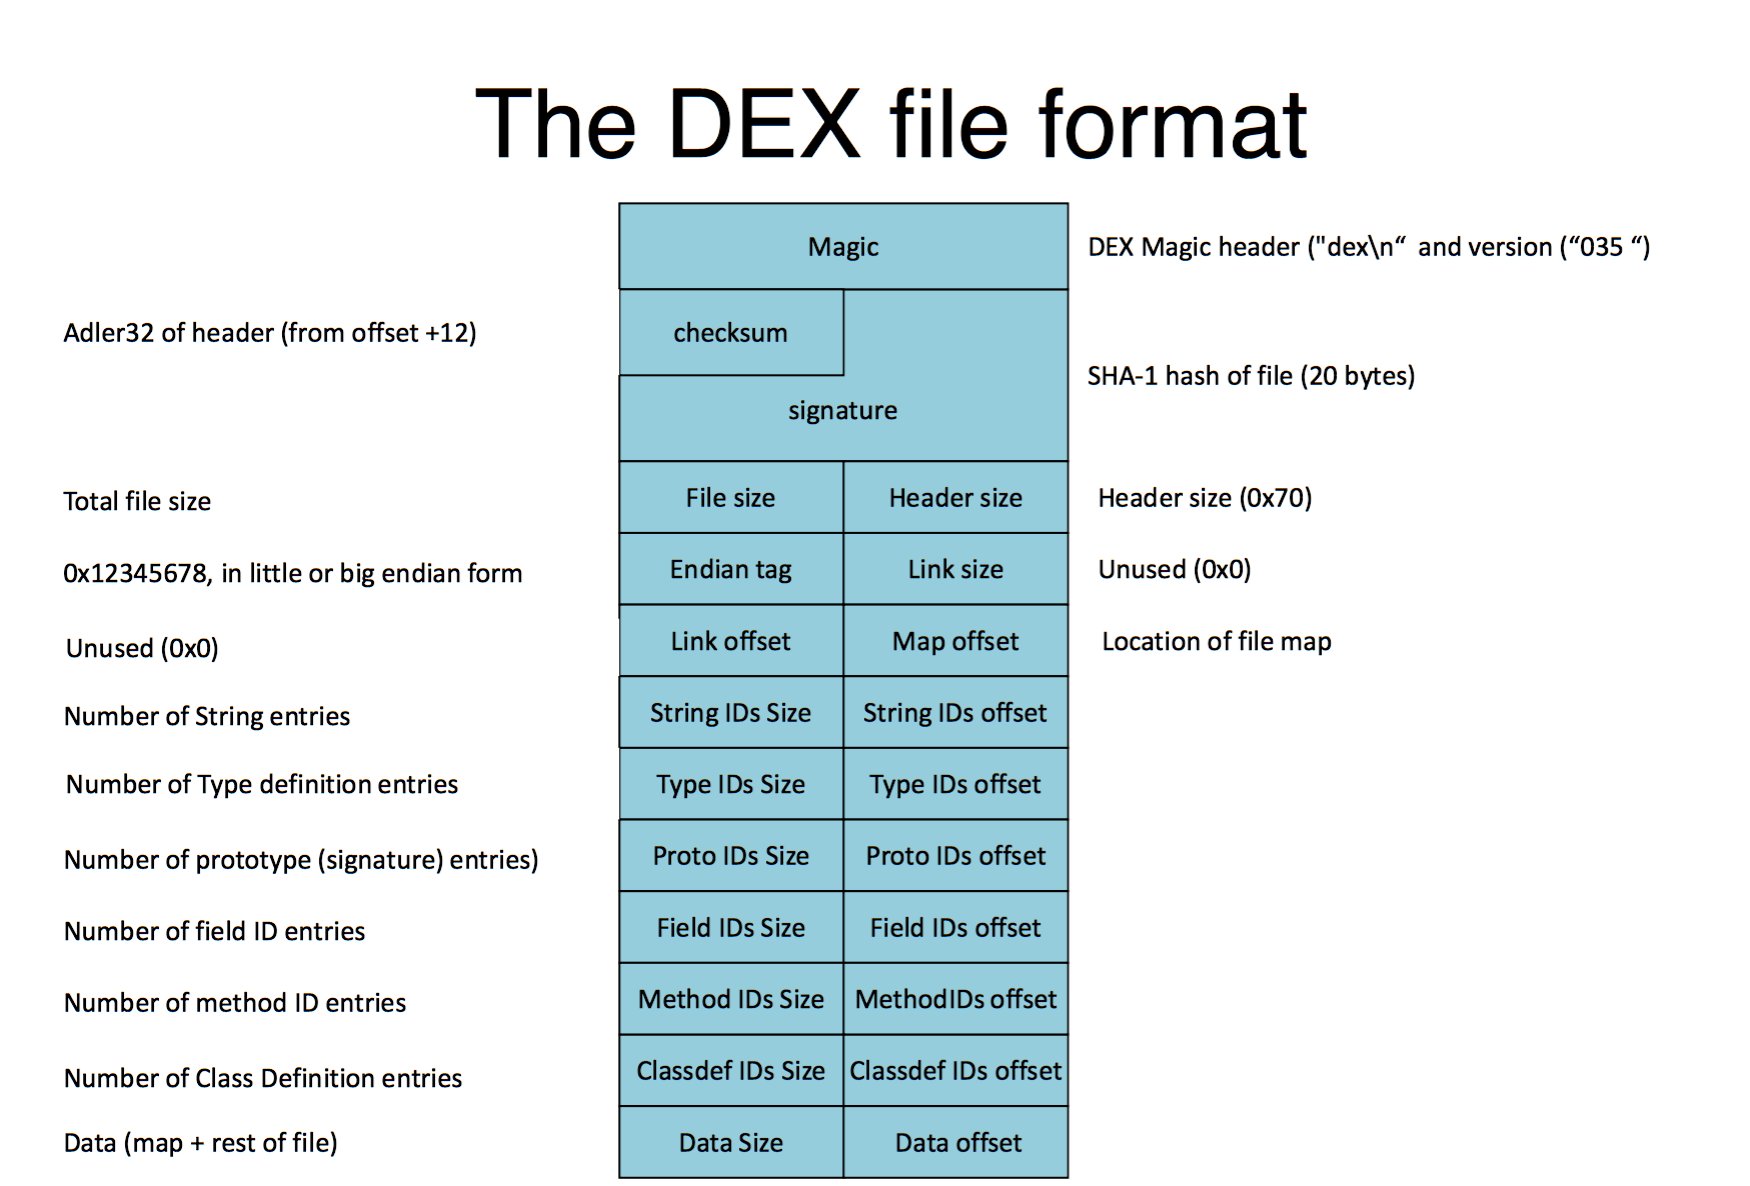
\includegraphics[width=0.8\textwidth]{data/dex1.png}
    \caption{dex1}
    \label{fig:dex1}
\end{figure}
\begin{figure}[h]
    \centering
    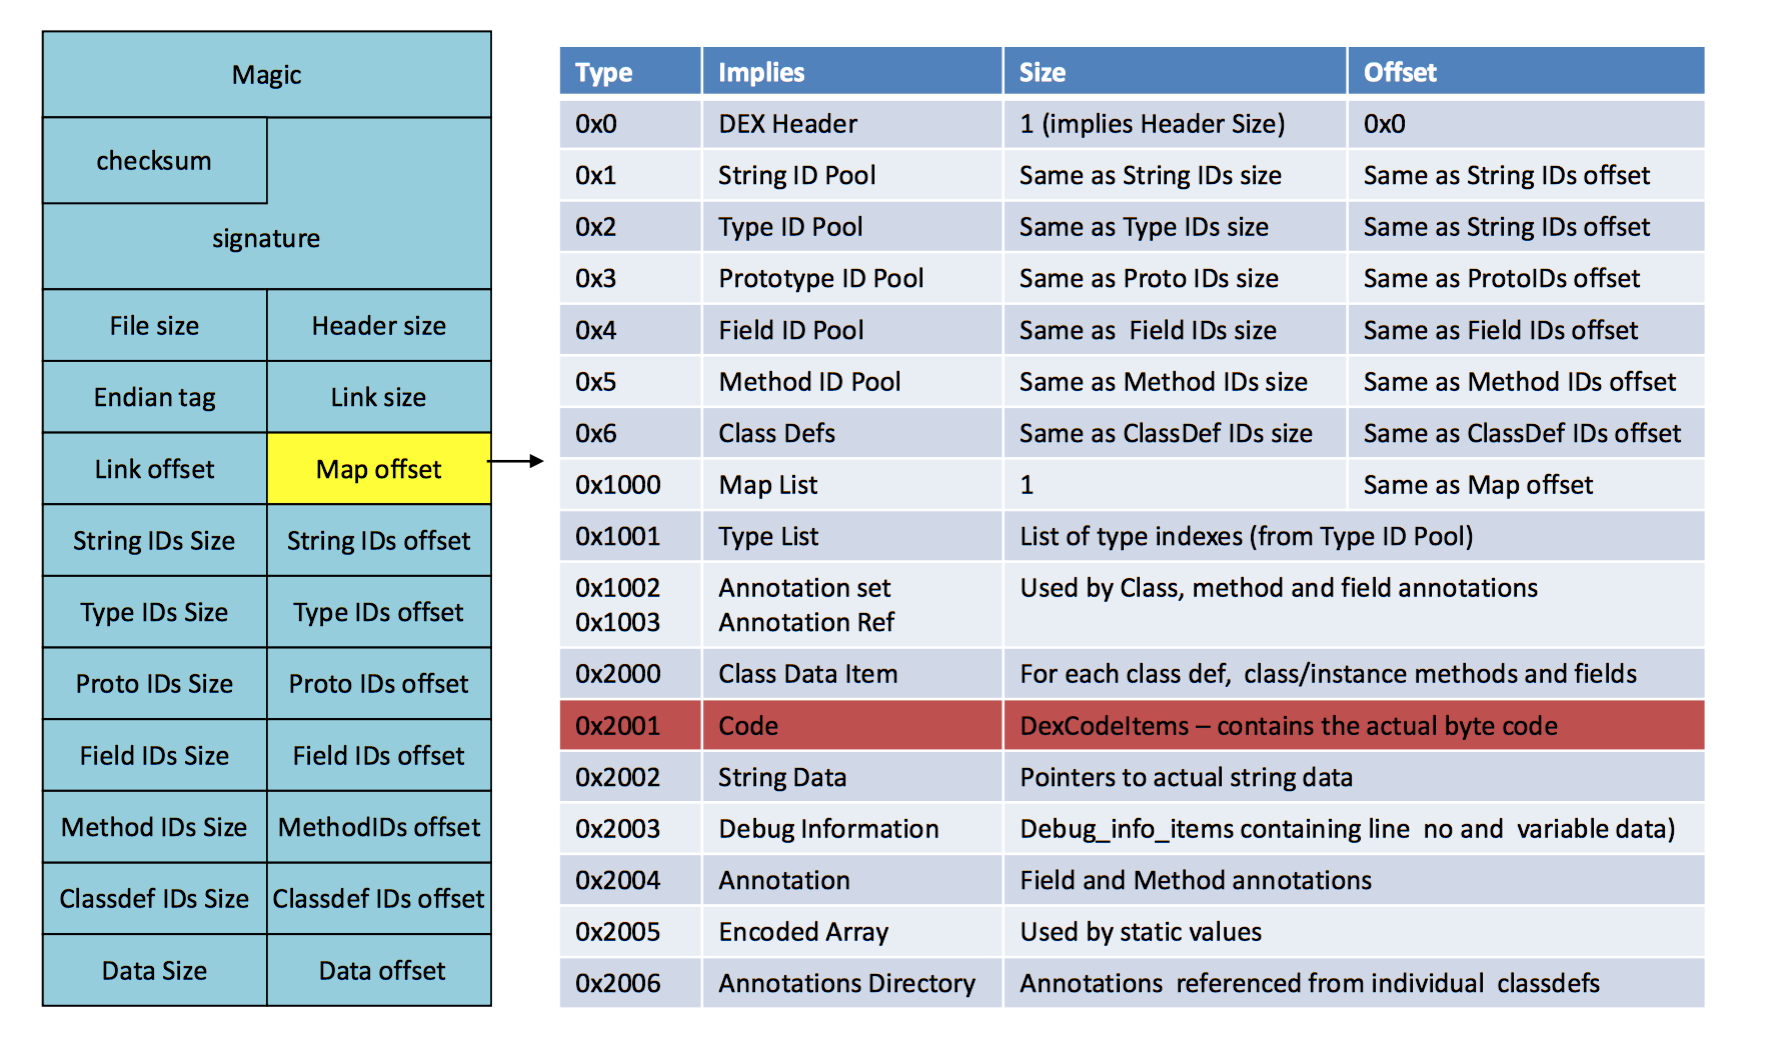
\includegraphics[width=0.8\textwidth]{data/dex2.png}
    \caption{dex2}
    \label{fig:dex2}
\end{figure}
dex instructions refer to indexes (in pools)\newline
de bytecode is striktly similar to java bytecode, allows for ease de/re compilation back and forth to/from java\newline

dex vs java\newline
java vm is stack based, dex is register based
java bytecode is actually more compact than dex
dex bytecode is more suited to arm architectures, mapping from dex registers to arm registers
dex supports bytecode optimizations, java no, apk's calsses.dex are optimized before install, on device\newline
\cite{andevconDalvikART}
%

AUFBAU DALVIK BYTECODE\newline
The program code of an Android application is delivered in form of Dalvik bytecode\newline
It will be executed by the Dalvik Virtual Machine and is comparable to Java bytecode. So there is a separate
optimizing step while installing an application, where the bytecode gets optimized for the underlaying architecture. The optimized form is also called ”odex”. The optimization is done by a program called ”dexopt” which is part of the Android platform. The DVM can execute optimized as well as not optimized Dalvik bytecode\newline

unterschied \url{http://newandroidbook.com/files/Andevcon-DEX.pdf}\newline

.dex file
The Dalvik bytecode consists of opcodes and is thus hard to read for humans. The Cracking Tool has to modify the opcodes in order to alter the behaviour of the application. Since it is directly read by the Dalvik virtual machine, it is the single point of truth.\newline

.odex file
Dalvik bytecode of an application is normally not optimized, because it is executed by a DVM which can run under different architectures\newline
